\fancyhead[LE]{\fontsize{8.5pt}{10pt}\selectfont\textbf{\textsf{\thepage}}\quad \textbf{\textsf{CHƯƠNG 1}}\quad \textsf{Các hàm số và Mô hình}}
\fancyhead[RO]{\fontsize{8.5pt}{10pt}\selectfont\textsf{MỤC 1.2}\quad \textbf{\textsf{\thepage}}}

\noindent
\begin{minipage}[t]{0.265\textwidth}
    \fontsize{8pt}{10pt}\selectfont
    \vspace*{35pt}
    \noindent
    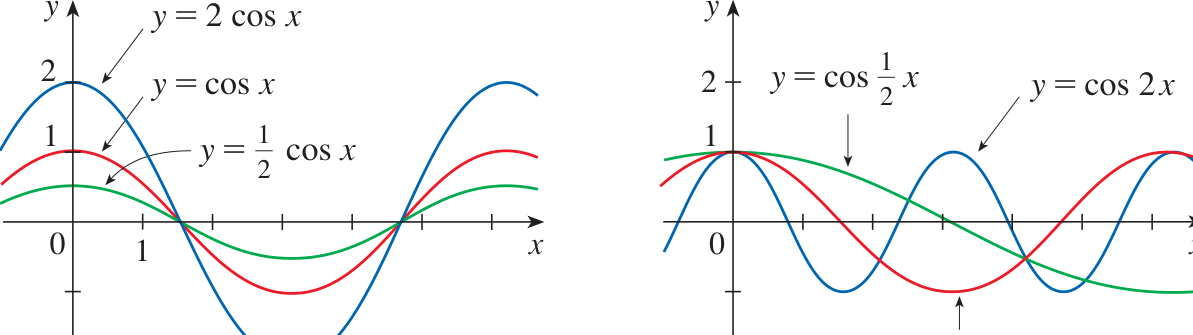
\includegraphics[width=0.92\linewidth]{images/p0073_fig3.png}
    \par\vspace{3pt}
    \textbf{\textsf{HÌNH 3}}

    \vspace{95pt}
    \noindent
    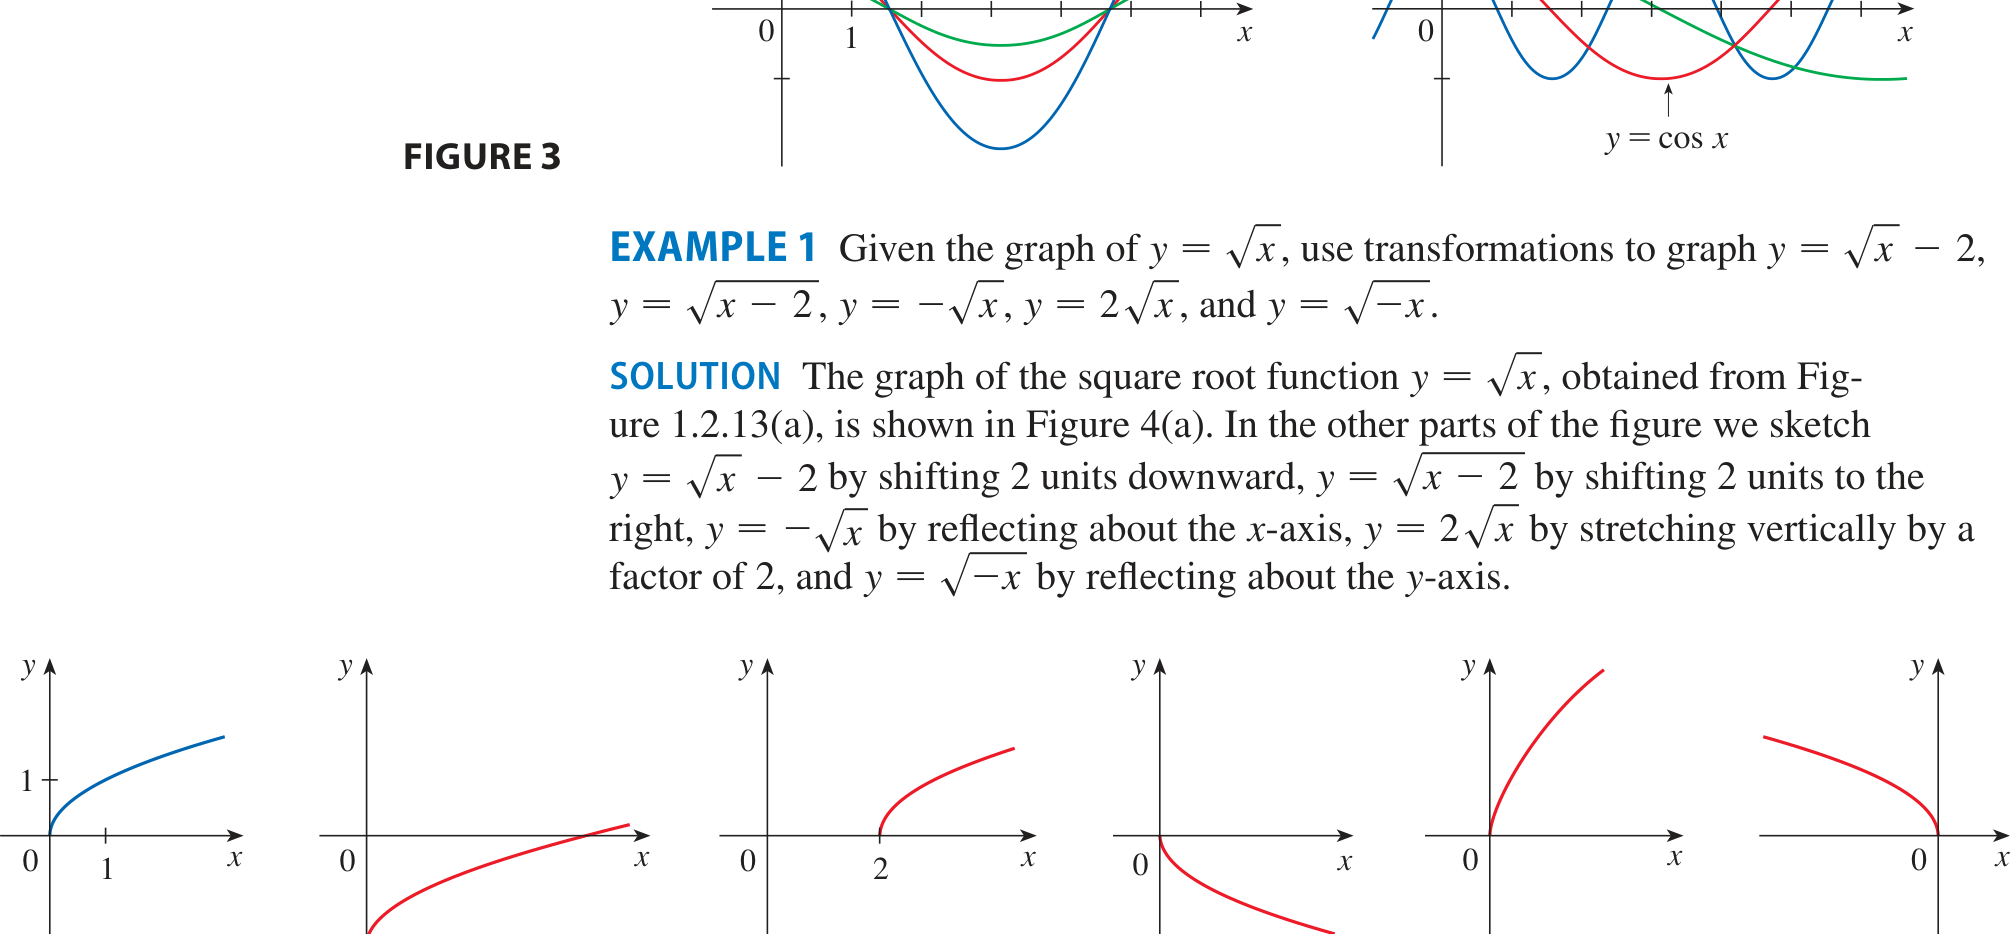
\includegraphics[width=0.92\linewidth]{images/p0073_fig4.png}
    \par\vspace{3pt}
    \textbf{\textsf{HÌNH 4}}

    \vspace{85pt}
    \noindent
    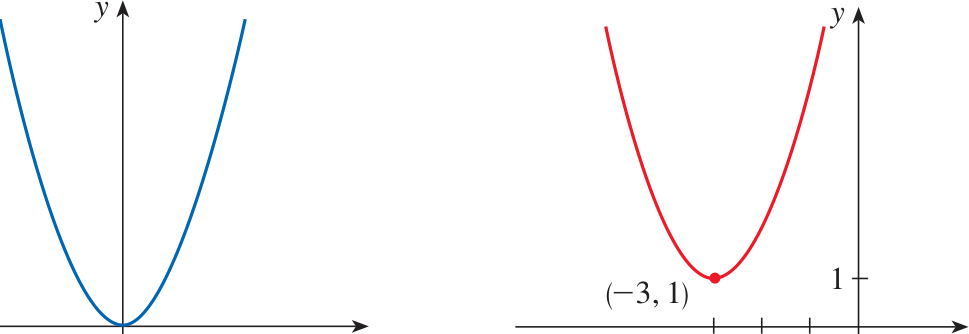
\includegraphics[width=0.92\linewidth]{images/p0073_fig5.png}
    \par\vspace{3pt}
    \textbf{\textsf{HÌNH 5}}
\end{minipage}%
\hfill
\begin{minipage}[t]{0.708\textwidth}
    \fontsize{9.3pt}{13.2pt}\selectfont
    Hình 3 minh họa các phép biến đổi co giãn này khi áp dụng cho hàm côsin với $c = 2$. Chẳng hạn, để nhận được đồ thị của $y = 2\cos x$, ta nhân tung độ $y$ của mỗi điểm trên đồ thị $y = \cos x$ với $2$. Điều này có nghĩa là đồ thị của $y = \cos x$ bị giãn theo phương thẳng đứng với hệ số $2$.

    \vspace{1.2em}
    \noindent
    \textbf{\textsf{\color{stewartcyan}VÍ DỤ 1}}\quad Cho đồ thị của $y = \sqrt{x}$, hãy sử dụng các phép biến đổi để vẽ đồ thị của $y = \sqrt{x} - 2$, $y = \sqrt{x - 2}$, $y = -\sqrt{x}$, $y = 2\sqrt{x}$ và $y = \sqrt{-x}$.

    \vspace{0.5em}
    \noindent
    \textbf{\textsf{\color{stewartcyan}LỜI GIẢI}}\quad Đồ thị của hàm căn bậc hai $y = \sqrt{x}$, nhận được từ Hình 1.2.13(a), được thể hiện trong Hình 4(a). Trong các phần còn lại của hình, ta vẽ đồ thị của $y = \sqrt{x} - 2$ bằng cách tịnh tiến $2$ đơn vị xuống dưới, $y = \sqrt{x - 2}$ bằng cách tịnh tiến $2$ đơn vị sang phải, $y = -\sqrt{x}$ bằng cách lấy đối xứng qua trục $x$, $y = 2\sqrt{x}$ bằng cách giãn theo phương thẳng đứng với hệ số $2$, và $y = \sqrt{-x}$ bằng cách lấy đối xứng qua trục $y$.\hfill{\color{stewartcyan}$\blacksquare$}

    \vspace{2.2em}
    \noindent
    \textbf{\textsf{\color{stewartcyan}VÍ DỤ 2}}\quad Vẽ đồ thị của hàm số $f(x) = x^2 + 6x + 10$.

    \vspace{0.5em}
    \noindent
    \textbf{\textsf{\color{stewartcyan}LỜI GIẢI}}\quad Bằng cách hoàn thành bình phương, ta viết phương trình của đồ thị dưới dạng
    \[
    y = x^2 + 6x + 10 = (x + 3)^2 + 1
    \]
    Điều này có nghĩa là ta nhận được đồ thị mong muốn bằng cách xuất phát từ parabol $y = x^2$ rồi tịnh tiến $3$ đơn vị sang trái và sau đó $1$ đơn vị lên trên (xem Hình 5).\hfill{\color{stewartcyan}$\blacksquare$}
\end{minipage}